\documentclass[conference]{IEEEtran}
\usepackage[pdftex]{graphicx}
\usepackage{url}

% correct bad hyphenation here
\hyphenation{op-tical net-works semi-conduc-tor}

\begin{document}
\title{Asynchronous Arbitration Primitives\\for New Generation of Circuits and Systems\vspace{-3mm}}
\author{\IEEEauthorblockN{Andrey Mokhov\IEEEauthorrefmark{1}, Danil Sokolov, Victor Khomenko, Alex Yakovlev}
\IEEEauthorblockA{Newcastle University, Newcastle upon Tyne, United Kingdom}
\IEEEauthorblockA{\IEEEauthorrefmark{1}\emph{Corresponding author}: \url{andrey.mokhov@ncl.ac.uk}}}

\maketitle

\begin{abstract}
This paper presents an overview of a family of asynchronous arbitration primitives designed
to increase the resilience and efficiency of the new generation of circuits and systems.
We cover primitives for synchronisation and decision-making with an emphasis on interfacing
analog and digital worlds, sampling of non-persistent signals, and efficient handling of
correlated sensor events.
\end{abstract}

% no keywords

\section{Introduction}

The new generation of circuits and systems is breaking conventional walls between
different timing, power and technology domains. Modern `synchronous' and `digital'
systems are emphatically asynchronous-at-large and analog-at-heart: they contain tens
to hundreds of timing and voltage domains, some even thousands~\cite{2017_bohnenstiehl_kilocore}.
Asynchronous arbitration primitives are now used both to orchestrate the communication
between different clock domains~\cite{2017_jiang_noc} and to control the analog-digital
interfaces in on-chip power regulators~\cite{2017_sokolov_a4a}.

% Asynchronous arbitration primitives are key to the
% resilience and efficiency of these systems.

This paper presents an overview of the recently developed asynchronous arbitration
primitives that address the problem of interfacing between hazardous and/or analog
worlds and hazard-free asynchronous circuits in a safe way. We cover synchronisation and
decision-making primitives in Sections~\ref{sec-sync} and~\ref{sec-decision}, respectively.
All of the presented circuit specifications and implementations have beed developed using
the open-source asynchronous design tool \textsc{Workcraft}~\cite{Workcraft_website} and are
publicly available under the MIT license~\cite{Arbitration_primitives_github}.

% Asynchronous arbiters are notoriously difficult to design, therefore it is essential to
% use a formal methods for the specification and verification of the ...
% Below we review the language for the formal specification
% of asynchronous circuits, which is used throughout the paper.

\subsection*{Formal specification of asynchronous circuits}\label{sec-stg}

Signal Transition Graphs~(STGs) are commonly used for the specification,
verification and synthesis of asynchronous circuits. See a comprehensive
background on STGs in~\cite{2002_cortadella_book}.

As a brief introduction, let us examine the STG specification shown in
Fig.~\ref{fig:wait}(left-middle). The STG specifies the behaviour
of a circuit with the inputs $\{\textsf{sig}, \textsf{ctrl}\}$
and the output \textsf{san}. Rising and falling \emph{signal transitions} are depicted by text
nodes, e.g. \textsf{sig+} corresponds to the signal \textsf{sig} switching from~0 to~1.
There are also \emph{dummy transitions}, such as \textsf{e}, which do not correspond to
changes of signal values (think of them as abstract events).
Input, output and dummy transitions are conventionally shown in red, blue and black
colour, respectively.

Directed arcs express the \emph{precedence} relation
between transitions, e.g. the arc $\textsf{san+} \longrightarrow \textsf{ctrl-}$ indicates
that the input \textsf{ctrl} goes low only after the output \textsf{san} goes high.
An arc can be \emph{marked} with a \emph{token}, shown as a black dot, to specify
the initial state of the circuit: the tokens before the transitions \textsf{sig+} and
\textsf{ctrl+} imply the initial state \textsf{sig=ctrl=san=0}.

A transition is \emph{enabled} to occur if it has tokens on each of its incoming
arcs, otherwise it is \emph{disabled}, e.g. \textsf{ctrl+} is enabled and \textsf{san-}
is disabled. When a transition occurs, it \emph{consumes} the tokens on its incoming arcs
are \emph{produces} them on its outgoing arcs, e.g. \textsf{ctrl+} moves the token to the
arc~$\textsf{ctrl+} \longrightarrow \textsf{e}$. Undirected arcs, called
\emph{read arcs}, are used to \emph{test} the existence of a token in a \emph{place}, shown as
a circle (think of it just as a placeholder for a token), e.g. the read arc
$\textsf{sig1} \frac{~~~~}{~} \textsf{e}$ allows the dummy \textsf{e} to occur only if
the place is marked, i.e. if \textsf{sig=1}.

A transition is \emph{persistent} if, once enabled, it will occur without first becoming
disabled. The dummy \textsf{e} is the only \emph{non-persistent} transition in the
example: \textsf{sig-} can disable it by consuming the token from \textsf{sig1}. Non-persistence
can manifest itself as a \emph{hazard} in the circuit, whereby a gate starts
switching but is stopped midway resulting in a short analog pulse.

% Signal transition loop\\
% Handshake\\

\begin{figure}
\begin{center}
    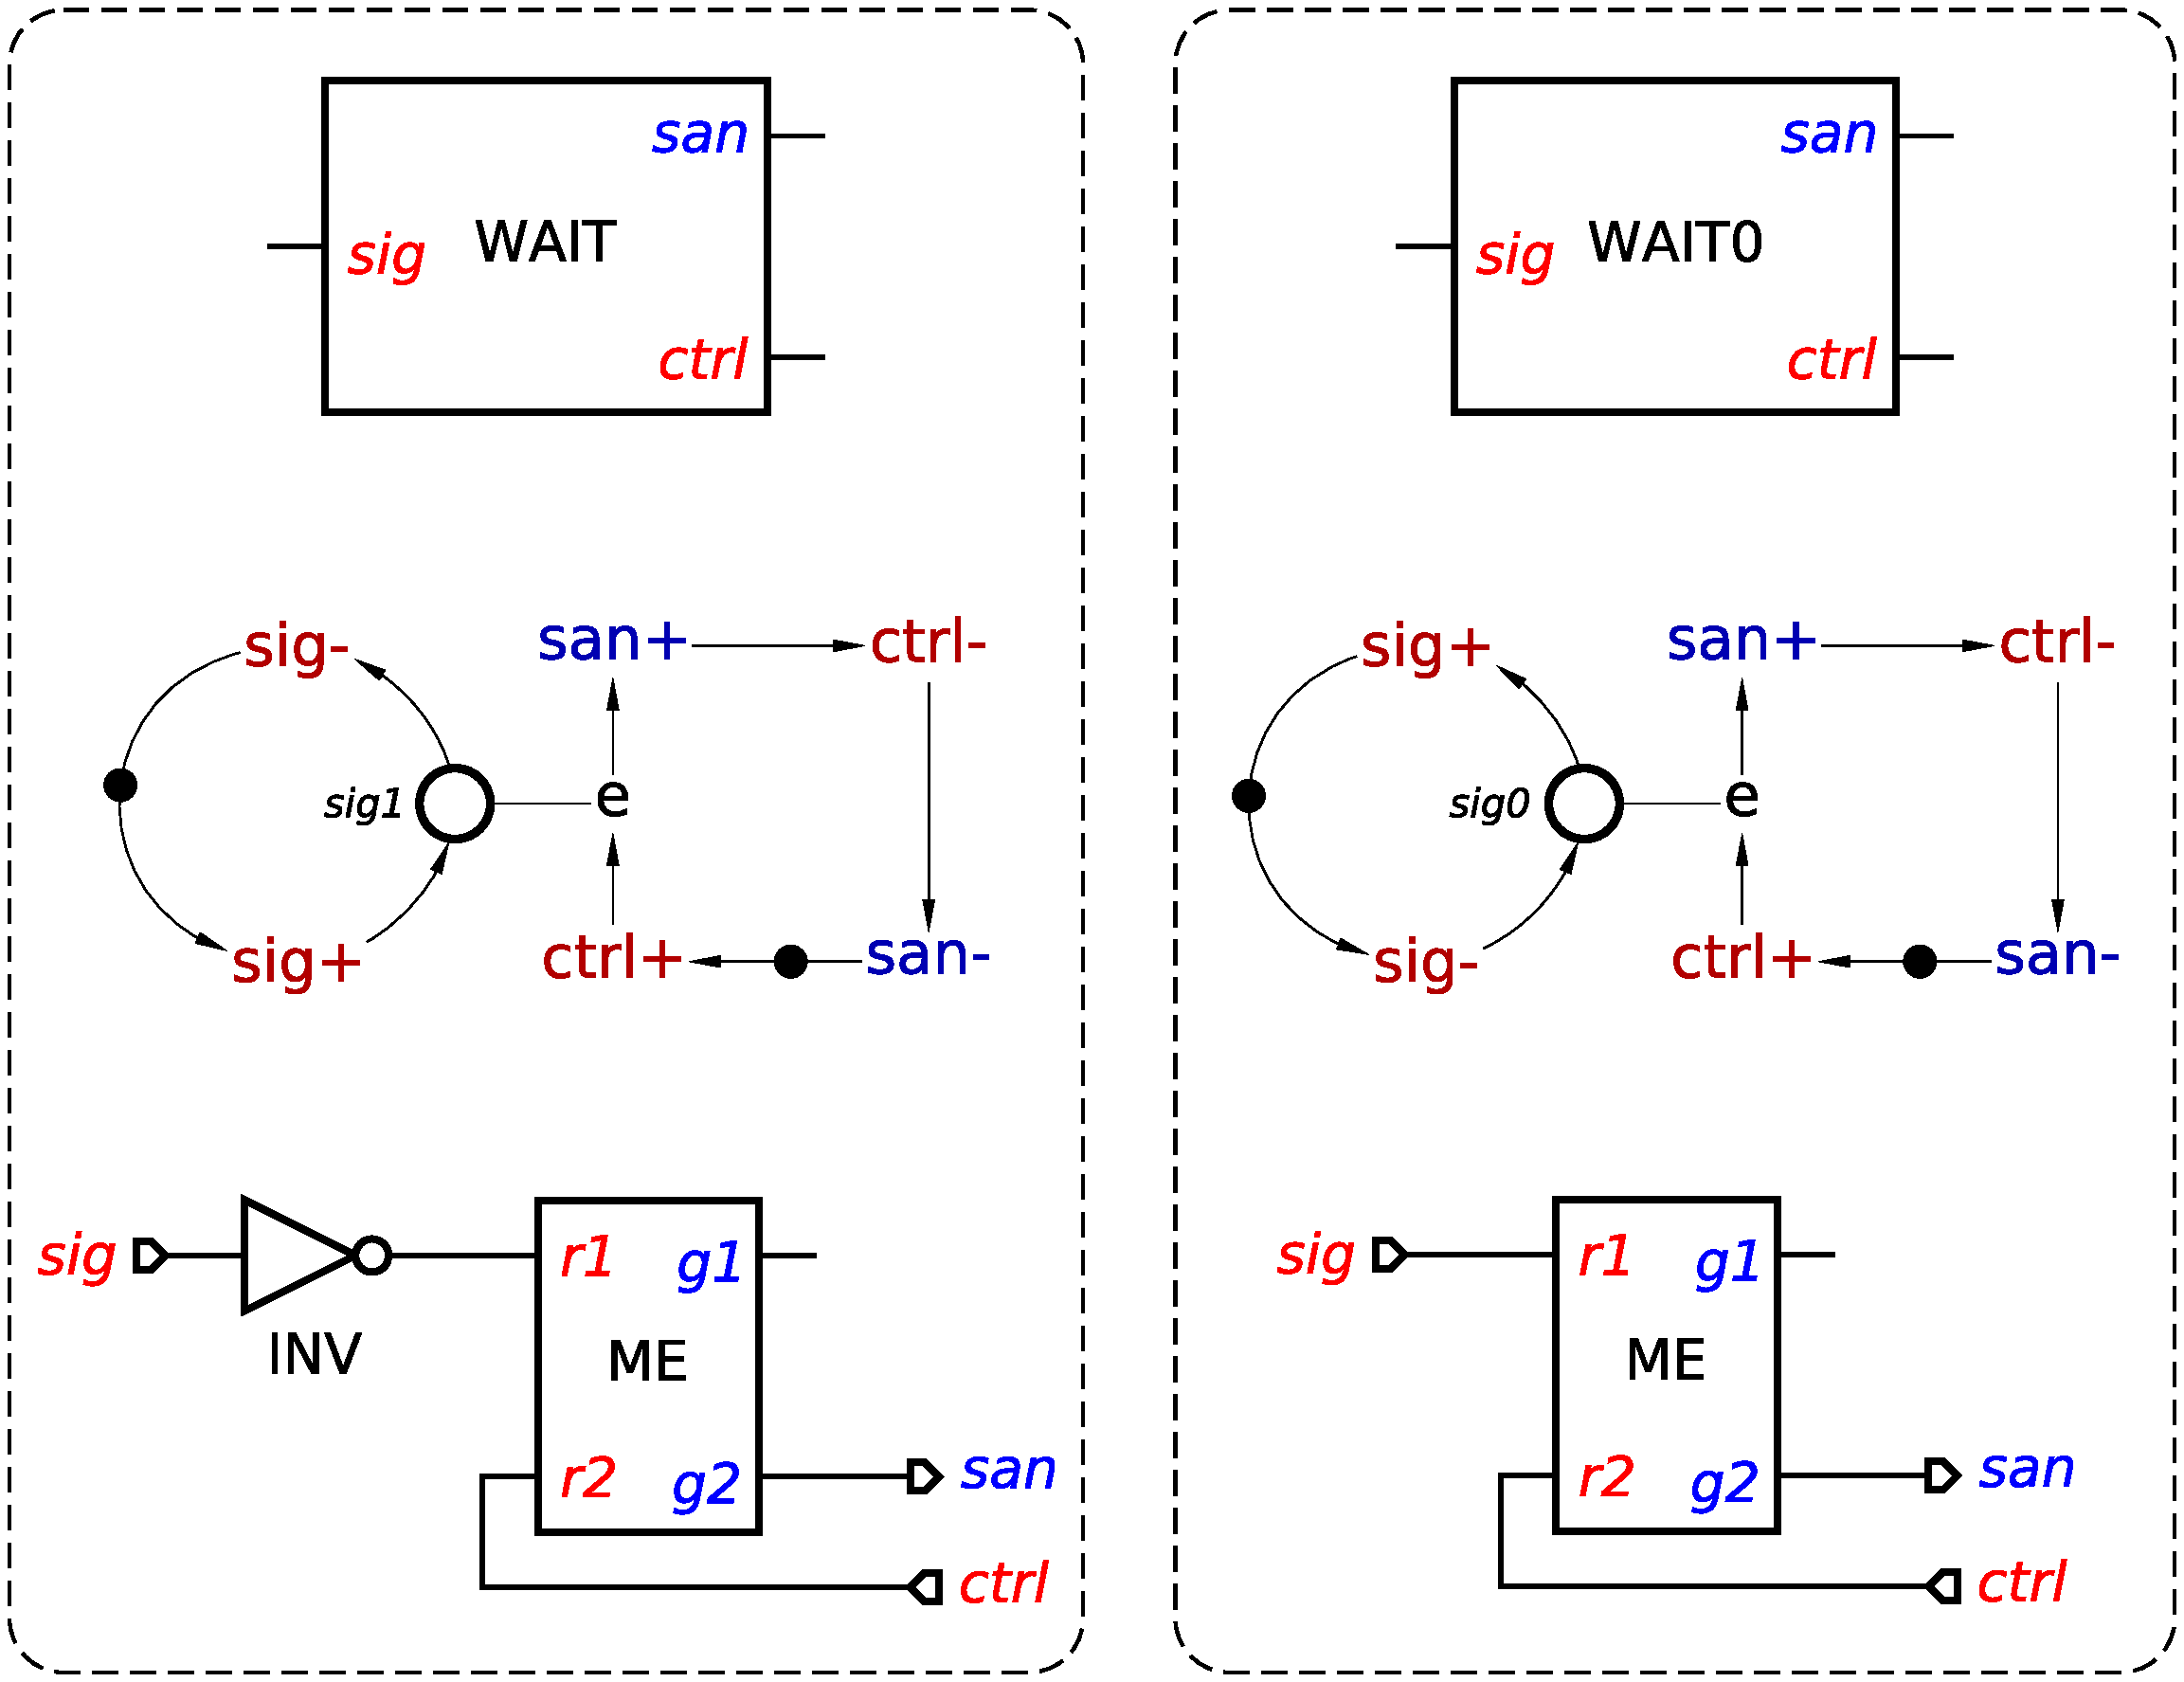
\includegraphics[scale=0.23]{fig/WAIT.pdf}
    \caption{\textsf{WAIT} and \textsf{WAIT0}: block diagram,
    specification and implementation.}
    \label{fig:wait}
    \vspace{-4mm}
\end{center}
\end{figure}

\section{Synchronisation primitives}\label{sec-sync}

This section covers the primitives for the synchronisation of hazard-free signal
transitions in asynchronous circuits with potentially hazardous signals coming
from the environment.
% Note: we use terms `hazard-free' and `persistent' as synonyms.

\subsection*{\textsf{WAIT} and \textsf{WAIT0}}

\begin{figure*}
\begin{center}
    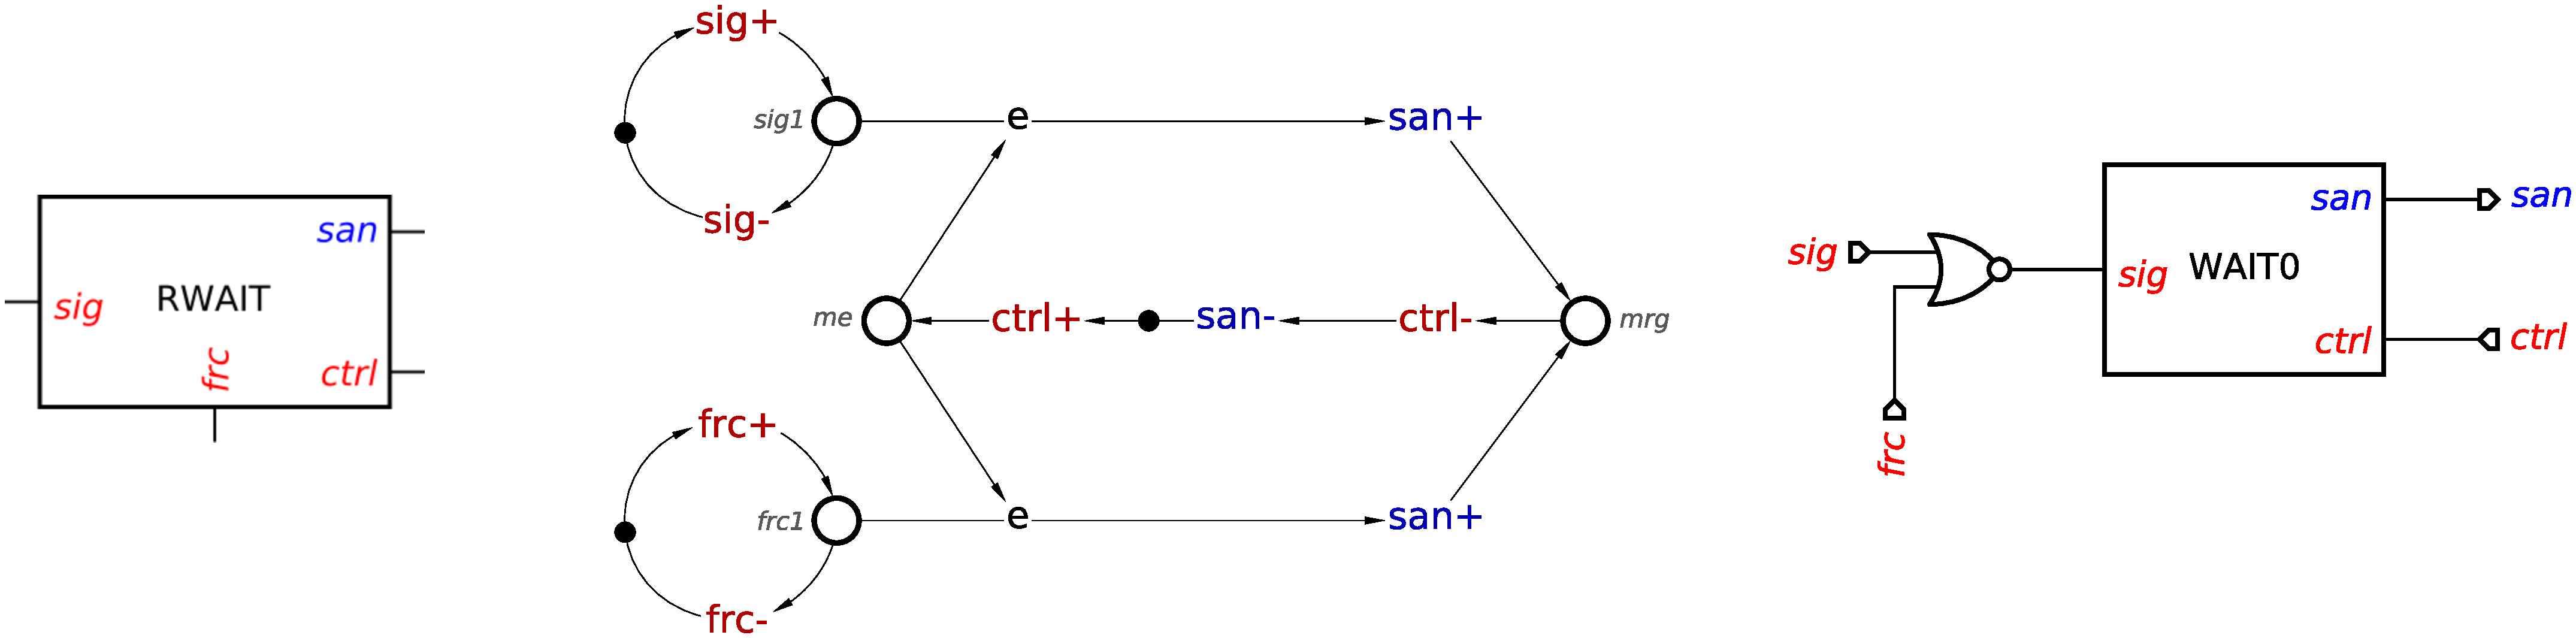
\includegraphics[scale=0.23]{fig/RWAIT.pdf}
    \vspace{-1mm}
    \caption{\textsf{RWAIT}: block diagram, specification and implementation.}
    \label{fig:rwait}
    \vspace{-5mm}
\end{center}
\end{figure*}

The \textsf{WAIT} element~\cite{2015_sokolov_multiphase}, shown in Fig.~\ref{fig:wait}(left),
synchronises the asynchronous handshake \textsf{ctrl/san} with the non-persistent
input~\textsf{sig}. According to the STG specification, \textsf{sig} is unconstrained and
is allowed to switch between~0 and~1 values with no regard to the output handshake -- this
is captured by the loop with signal transitions \textsf{sig+} and \textsf{sig-}.
Initially~\textsf{ctrl=0} and the input is isolated from the output \textsf{san}.
By switching the~\textsf{ctrl} input, the element is switched into the \emph{waiting mode},
where it stays until~\textsf{sig} becomes high and enables the
dummy~\textsf{e}. The output~\textsf{san=1} is then produced and persistently
held\footnote{Here and further on, the output \textsf{san}
is the `sanitised' (persistent) version of the `dirty' (non-persistent) input \textsf{sig}.}
until \textsf{WAIT} is reset by releasing the \textsf{ctrl} input (the transition~\textsf{ctrl-}).

Note that an input spike (\textsf{sig+} followed by \textsf{sig-}) in the waiting
mode can be too short fot the \textsf{WAIT} element to register it, in which case the spike
is ignored. The non-persistent behaviour and the associated metastability is fully contained
within the element, guaranteeing a clean hazard-free output. This is achieved using the
\emph{mutual-exclusion} \textsf{ME} element~\cite{2008_kinniment_synchronisation}.

\textsf{WAIT} is a fundamental synchronisation primitive that is used for
implementing other, more sophisticated components presented in this paper.
The symmetric version of the element that waits for the input to become low is
called \textsf{WAIT0}; its top-level block diagram, the STG specification and
the implementation are shown in Fig.~\ref{fig:wait}(right).

\subsection*{\textsf{RWAIT} and \textsf{RWAIT0}}

\textsf{RWAIT} and \textsf{RWAIT0} are modifications of the \textsf{WAIT} and \textsf{WAIT0}
elements, respectively, with a possibility to persistently cancel the waiting request. This
is useful when the input is no longer expected to change or the change is no longer relevant
for the asynchronous controller, and hence the output handshake needs to be released.

See the block diagram of \textsf{RWAIT} in Fig.~\ref{fig:rwait}. The additional input
\textsf{frc} can be used to force the reset of the output handshake in the waiting mode. The
STG specifies that the output transition \textsf{san+} can be caused either by~\textsf{sig+}
(the top branch) or by~\textsf{frc+}~(the bottom branch). The implementation reflects the resulting
OR-causality~\cite{1996_yakovlev_or}: the inputs \textsf{sig} and \textsf{frc} are simply
combined via a NOR gate, whose output is synchronised with the handshake \textsf{ctrl/san}
using the \textsf{WAIT0} element.

% The \textsf{RWAIT0} element is implemented analogously.

\subsection*{\textsf{WAIT01} and \textsf{WAIT10}}

\textsf{WAIT01} and \textsf{WAIT10} elements wait for a rising or falling edge of the input
signal, respectively. Note that this is subtly different from waiting for high or low input value,
e.g. a signal can be initially low, and to generate a falling edge event it must first go high.
The \textsf{WAIT01} specification in Fig.~\ref{fig:wait012}(left-middle) tracks the input changes
via two dummy transitions that are enabled in sequence when \textsf{sig=0} and \textsf{sig=1} hold.
This can be implemented by connecting \textsf{WAIT0} and \textsf{WAIT} in sequence.

An element waiting for an arbitrary fixed pattern of values, e.g. the symmetric
\textsf{WAIT10}, can be implemented analogously.

\begin{figure}
\begin{center}
    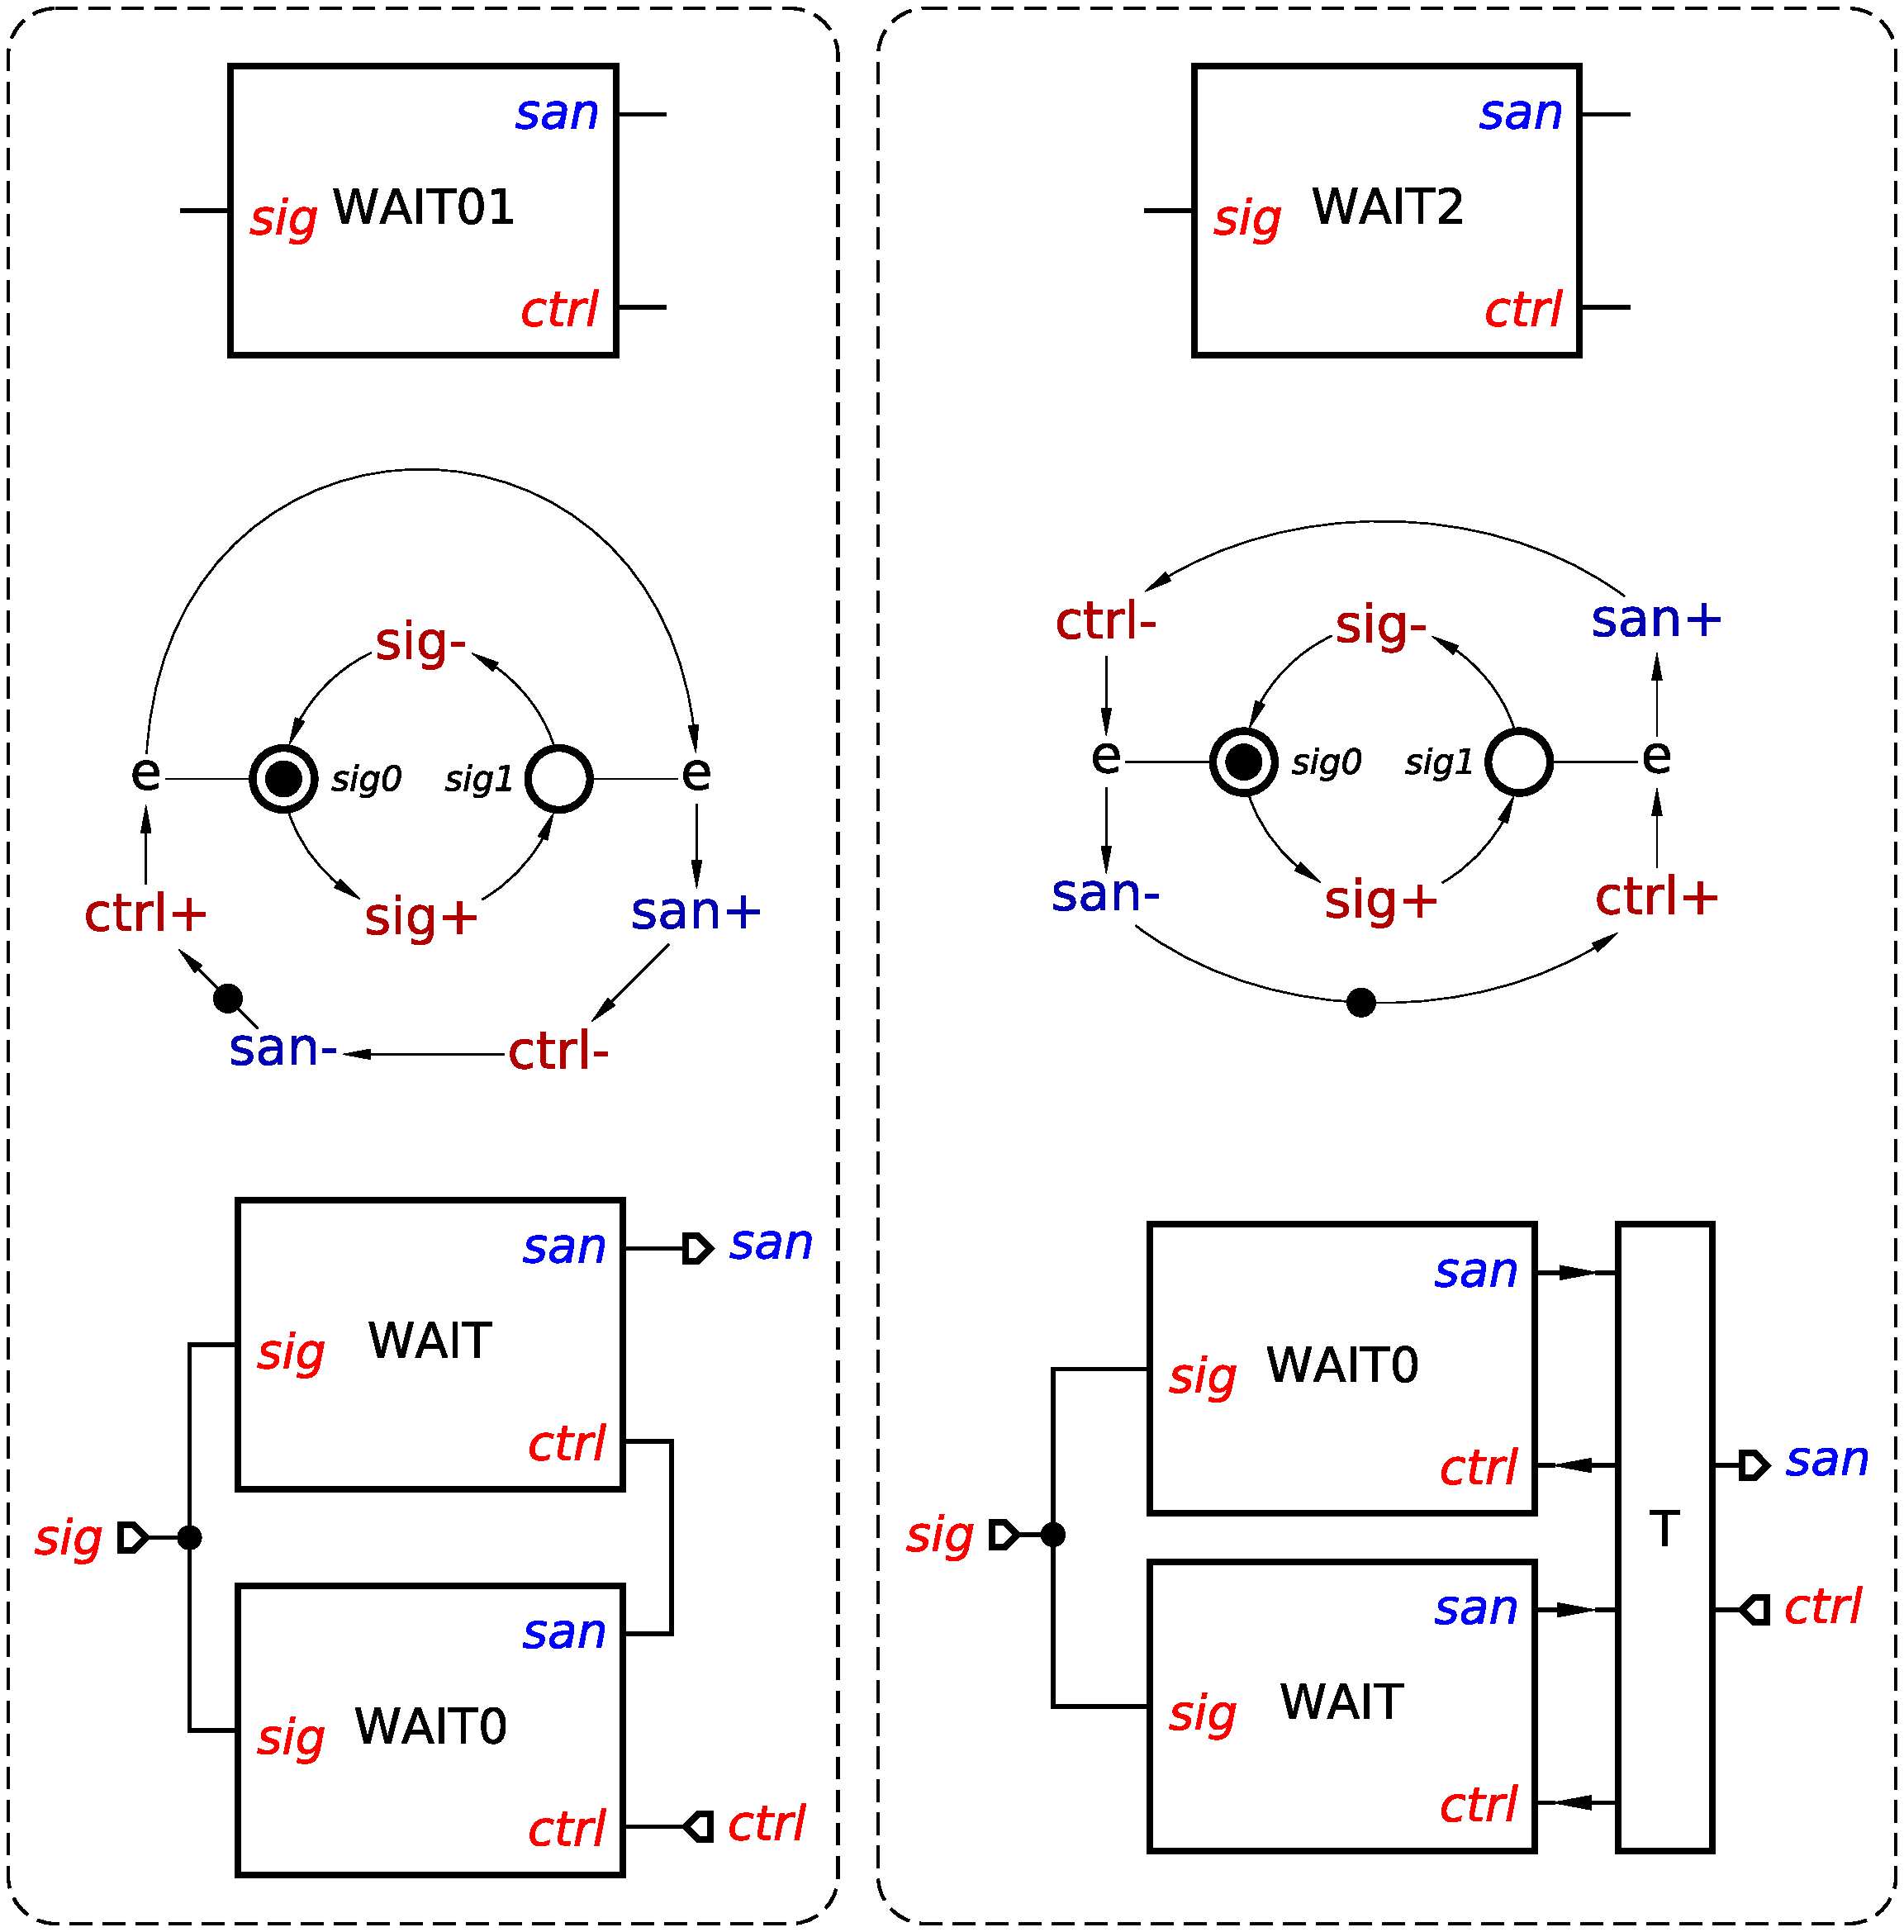
\includegraphics[scale=0.23]{fig/WAIT01-and-WAIT2.pdf}
    \caption{\textsf{WAIT01} and \textsf{WAIT2}: block diagram,
    specification, implementation.}
    \label{fig:wait012}
    \vspace{-4mm}
\end{center}
\end{figure}

\subsection*{\textsf{WAIT2}}

\textsf{WAIT2} is another combination of \textsf{WAIT} and \textsf{WAIT0} elements:
it uses a 2-phase output handshake, waiting for high and low input values, one after
the other, see Fig.~\ref{fig:wait012}(right).

The STG contains two loops: the inner \textsf{sig} loop, which is unconstrained, and
the outer handshake loop that synchronises the rising
($\textsf{ctrl+} \longrightarrow \textsf{san+}$)
 and the falling
($\textsf{ctrl-} \longrightarrow \textsf{san-}$)
phases with conditions \textsf{sig=1} and \textsf{sig=0}, respectively.

The implementation uses a toggle-like component \textsf{T}, which steers the rising and
falling edges of \textsf{ctrl} to the two four-phase output handshakes controlling
the \textsf{WAIT} and \textsf{WAIT0} elements. It is a standard
asynchronous component, and its implementation is beyond the scope of this paper.

\begin{figure*}
\begin{center}
    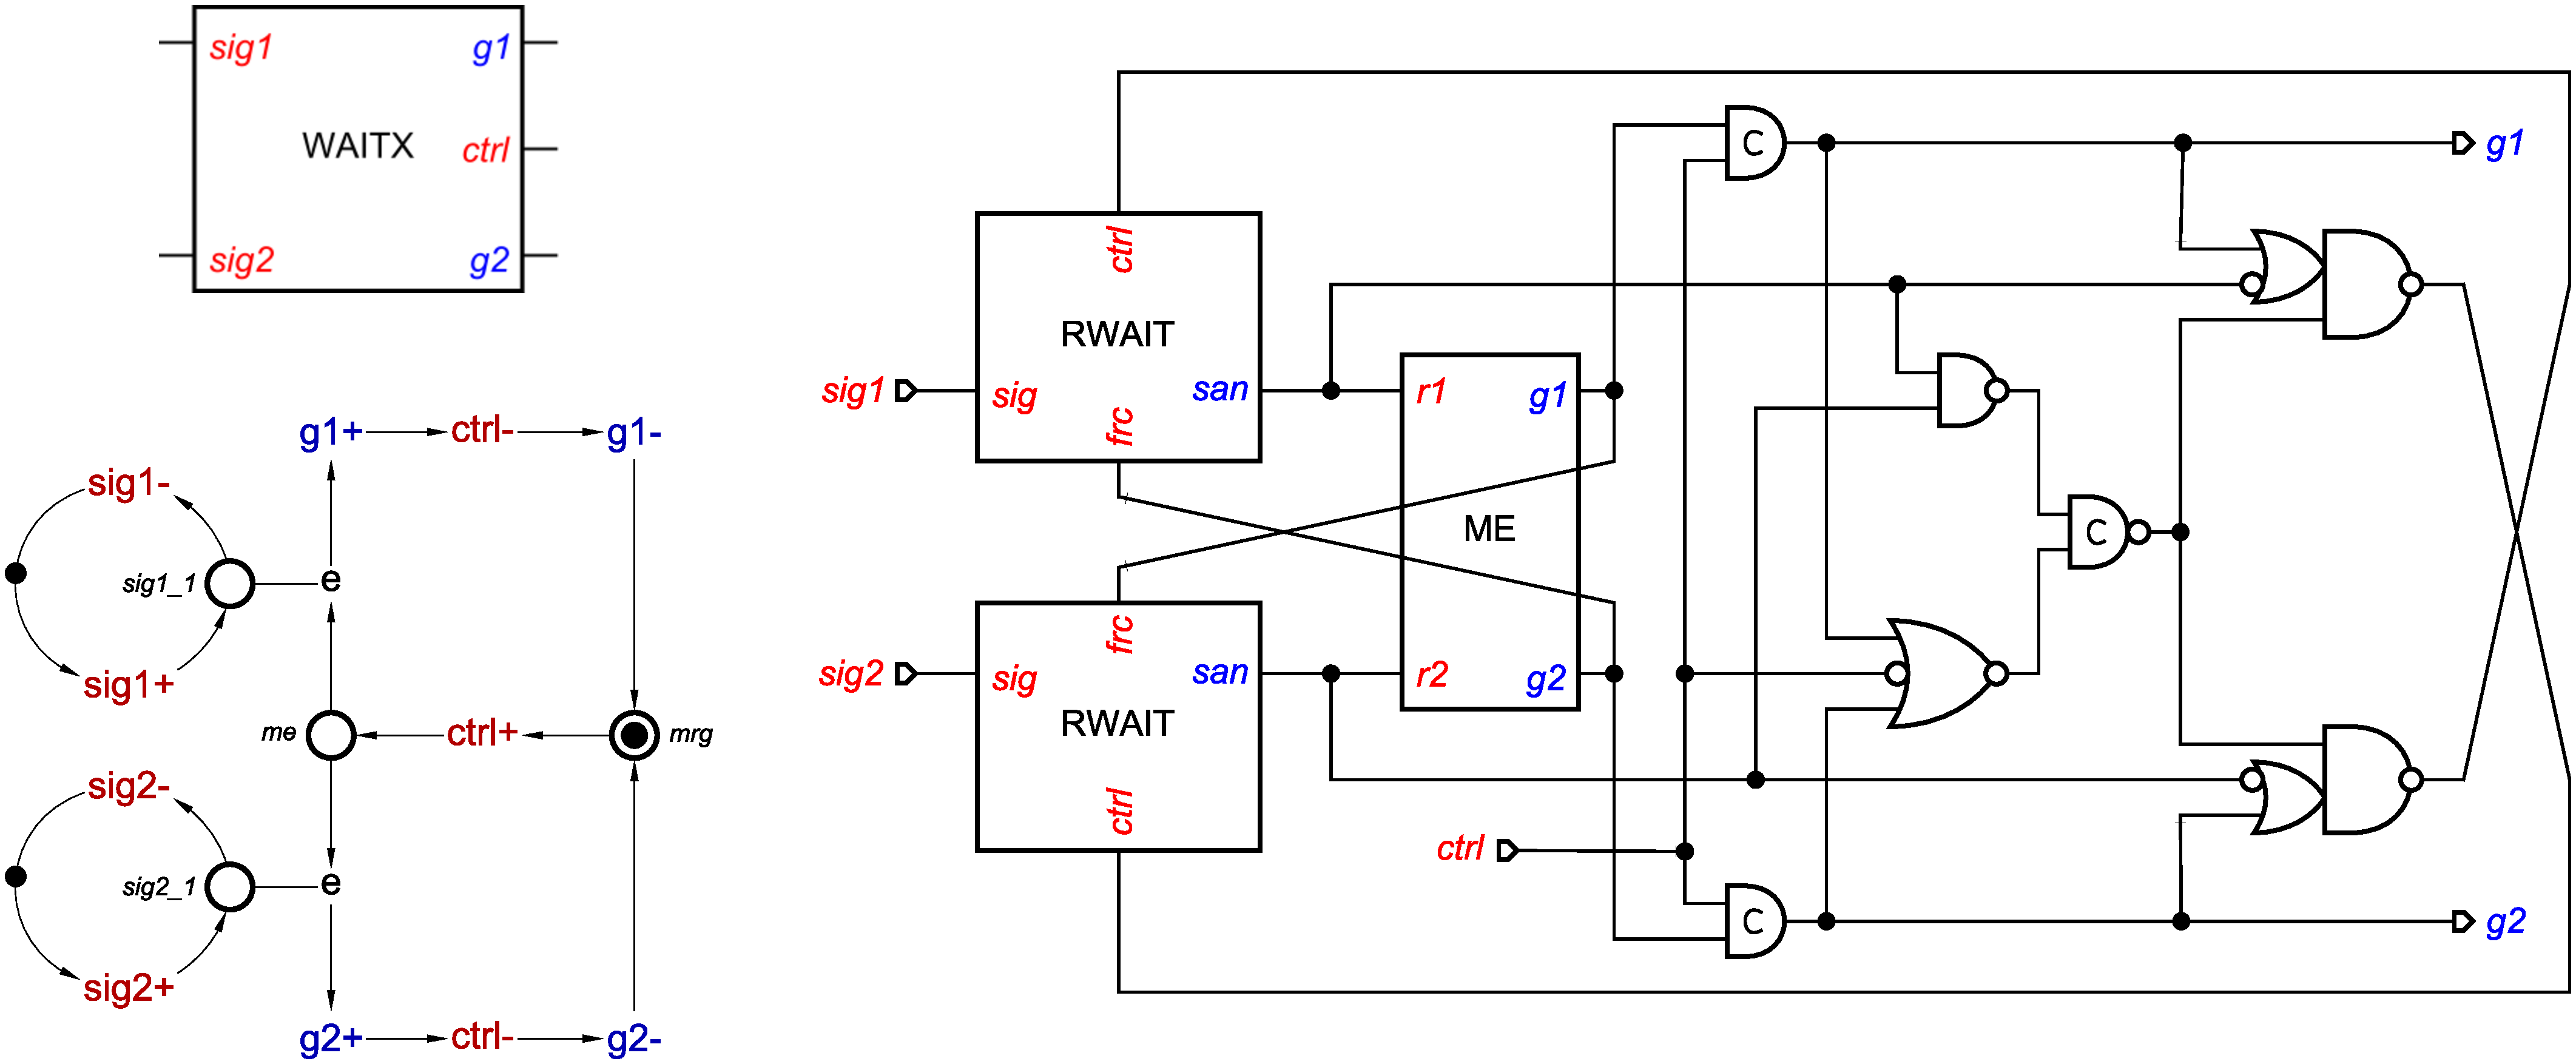
\includegraphics[scale=0.23]{fig/WAITX.pdf}
    \vspace{-2mm}
    \caption{\textsf{WAITX}: block diagram, specification and implementation.}
    \label{fig:waitx}
    \vspace{-6mm}
\end{center}
\end{figure*}

\section{Decision-making primitives}\label{sec-decision}

This section presents a family of \emph{decision-making} components that perform
non-trivial event coordination and rely on the previously introduced synchronisation
primitives.

\subsection*{\textsf{WAITX}}

The \textsf{WAITX} element~\cite{2017_khomenko_waitx} arbitrates between two
non-persistent inputs $\{\textsf{sig1}, \textsf{sig2}\}$, producing a clean
asynchronous dual-rail handshake: depending on which of the two signals arrives
first, exactly one of the grant signals $\{\textsf{g1}, \textsf{g2}\}$ is issued, see
Fig.~\ref{fig:waitx}. The place \textsf{me} with two consuming arcs represents to
the arbitration decision that needs to be made: if the inputs arrive very close to
each other, both of the two dummy transitions can become enabled but only one
of them can occur, since \textsf{me} can have at most one token. In the reset phase
both branches are merged in the place \textsf{mrg}.

\textsf{WAITX} isolates the outputs
both from the metastability associated with non-persistent inputs, as well as from
the metastability associated with making the decision of which input signal arrives first.
The implementation relies on \textsf{RWAIT} elements for synchronisation with
non-persistent signals, and uses an \textsf{ME} element to make the decision on their
arrival order.

\subsection*{\textsf{WAITX2}}

\begin{figure}
\begin{center}
    \vspace{-2mm}
    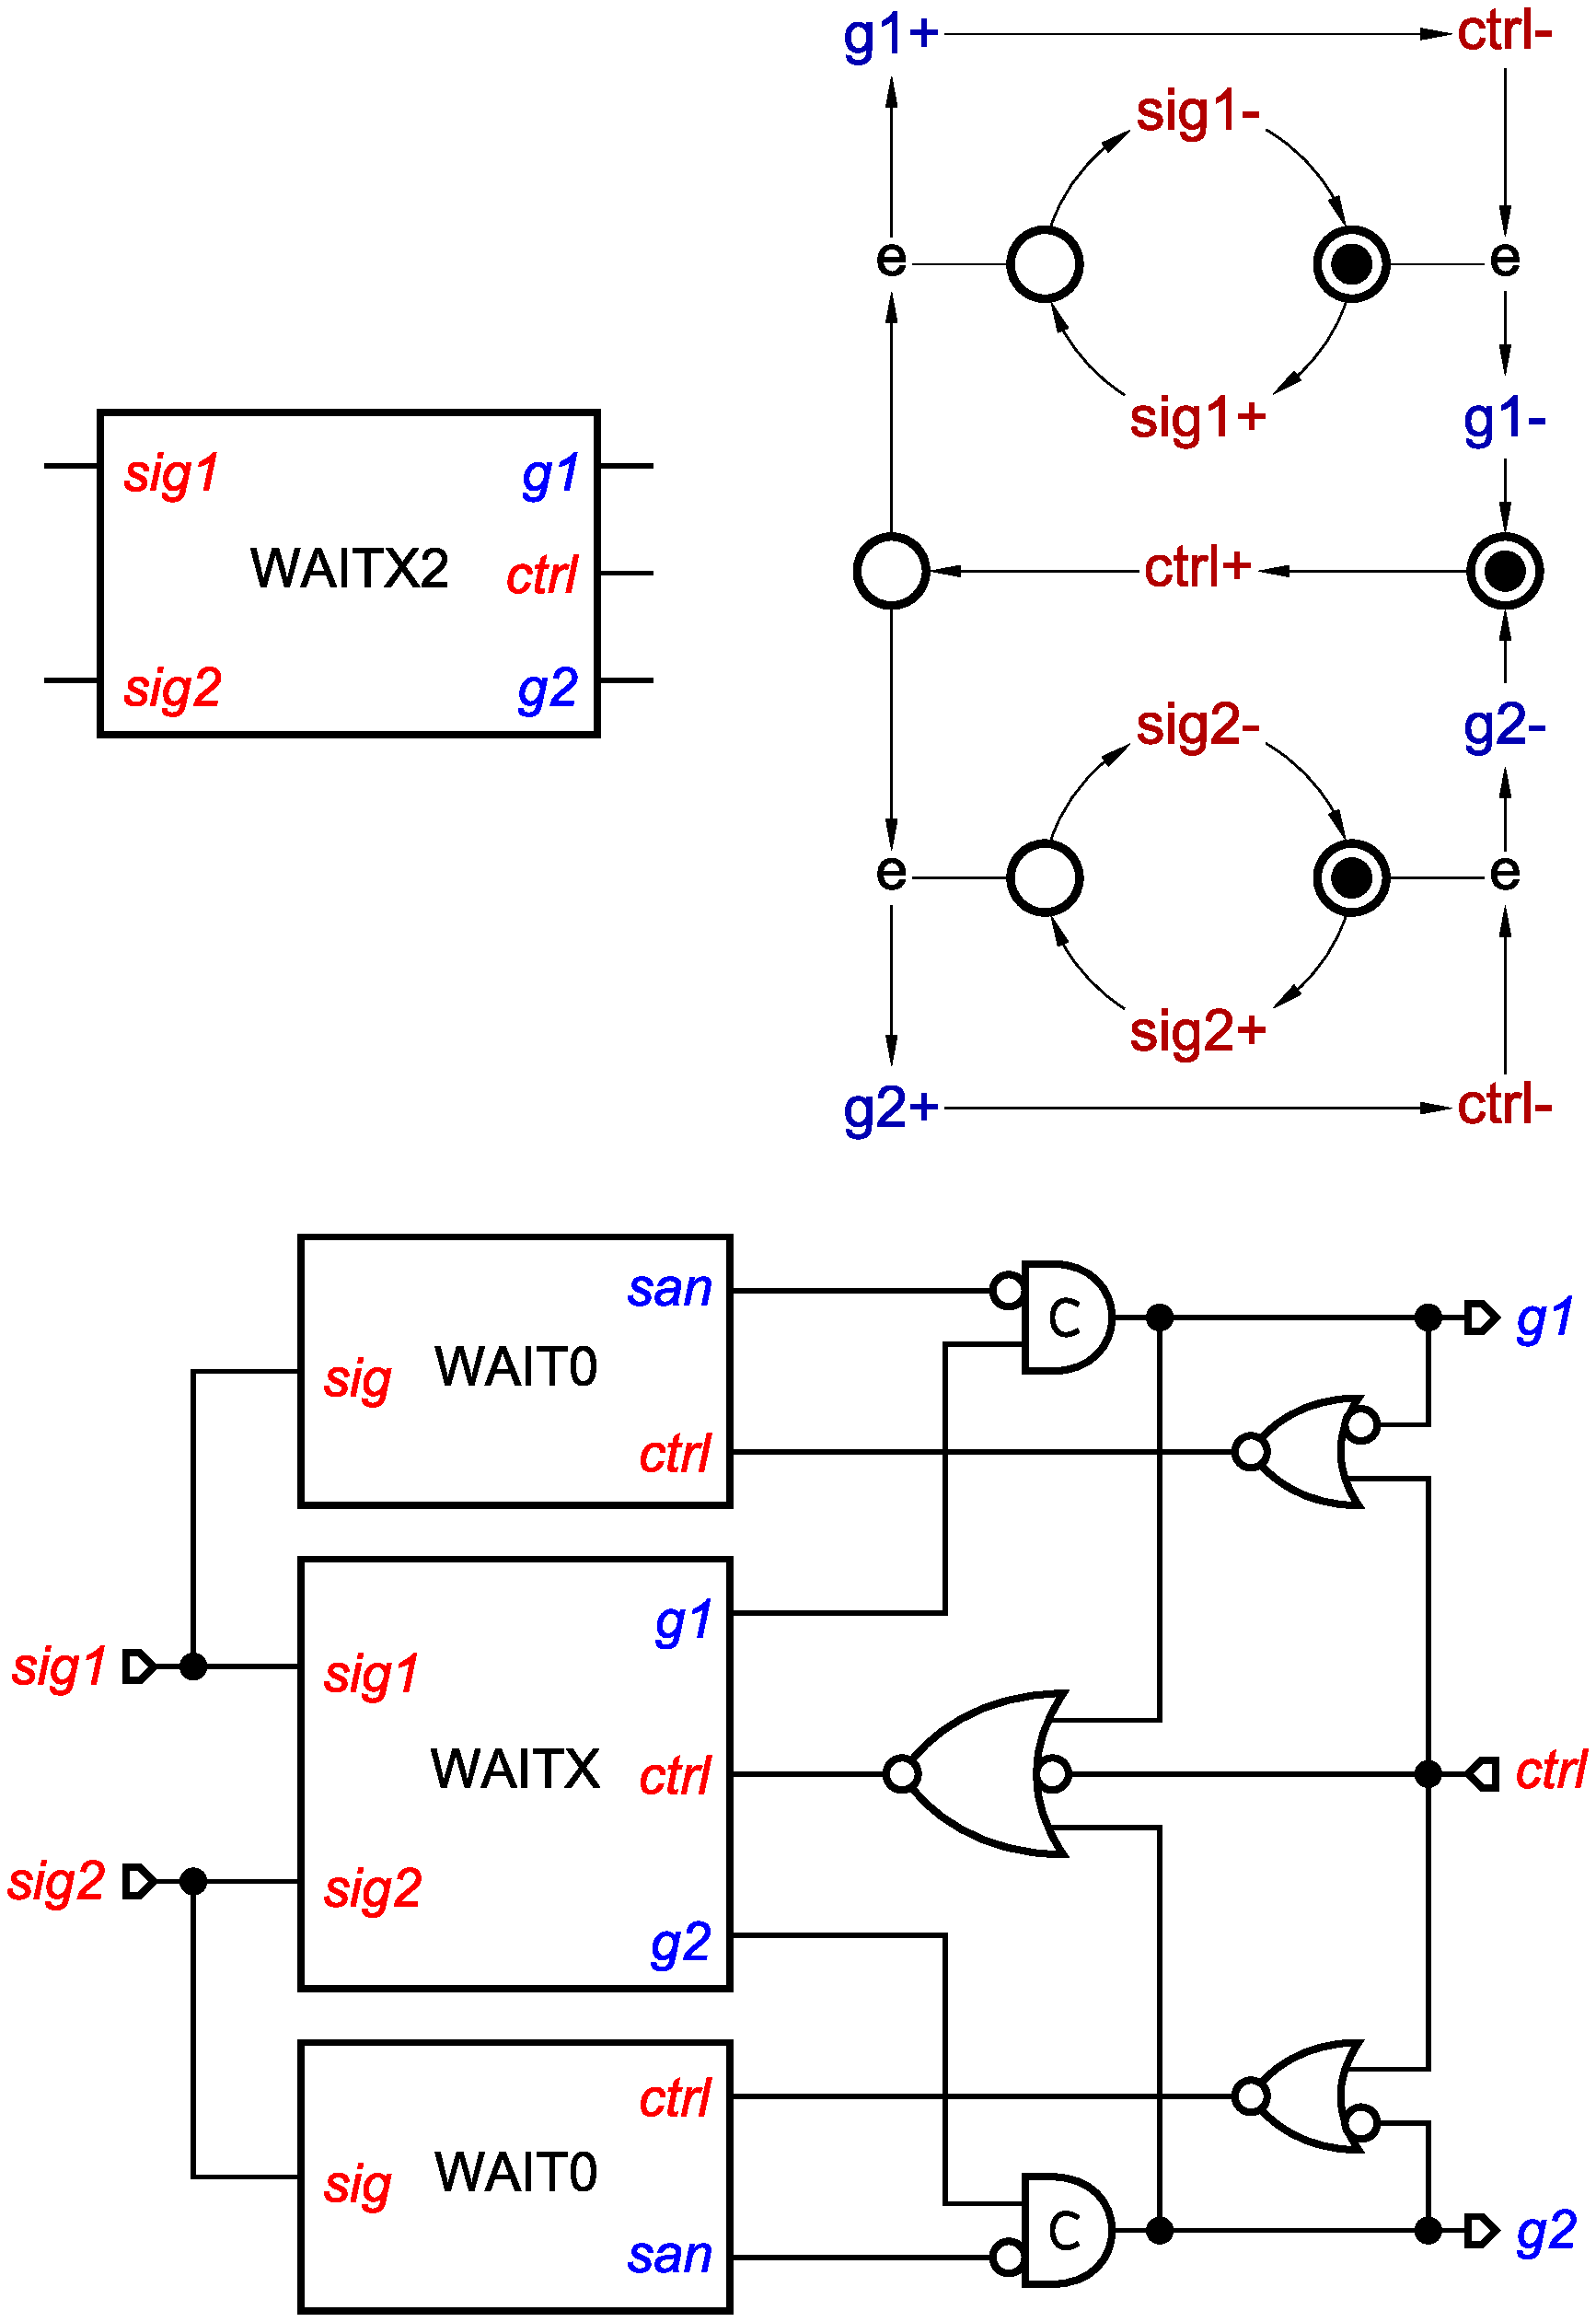
\includegraphics[scale=0.23]{fig/WAITX2.pdf}
    \caption{\textsf{WAITX2}: block diagram, specification and implementation.}
    \label{fig:waitx2}
    \vspace{-5mm}
\end{center}
\end{figure}

\textsf{WAITX2} behaves as \textsf{WAITX} in the rising phase and as \textsf{WAIT0}
in the falling phase, i.e. it does not release the output asynchronous handshake until
the winning input signal goes low. It uses a 2-phase output handshake similarly to
\textsf{WAIT2}, and the specification, shown in Fig.~\ref{fig:waitx2}, is therefore
a combination of the STGs for \textsf{WAITX} and \textsf{WAIT2}.

The implementation comprises \textsf{WAITX} and two \textsf{WAIT0} elements controlled
by toggle-like asynchronous logic, which activates the right \textsf{WAIT0} element in the
reset phase. The synthesis and technology mapping of the control was performed using
conventional asynchronous design approaches automated in
\textsc{Workcraft}~\cite{2017_sokolov_a4a}.

\subsection*{\textsf{SAMPLE}}

\begin{figure}
\begin{center}
    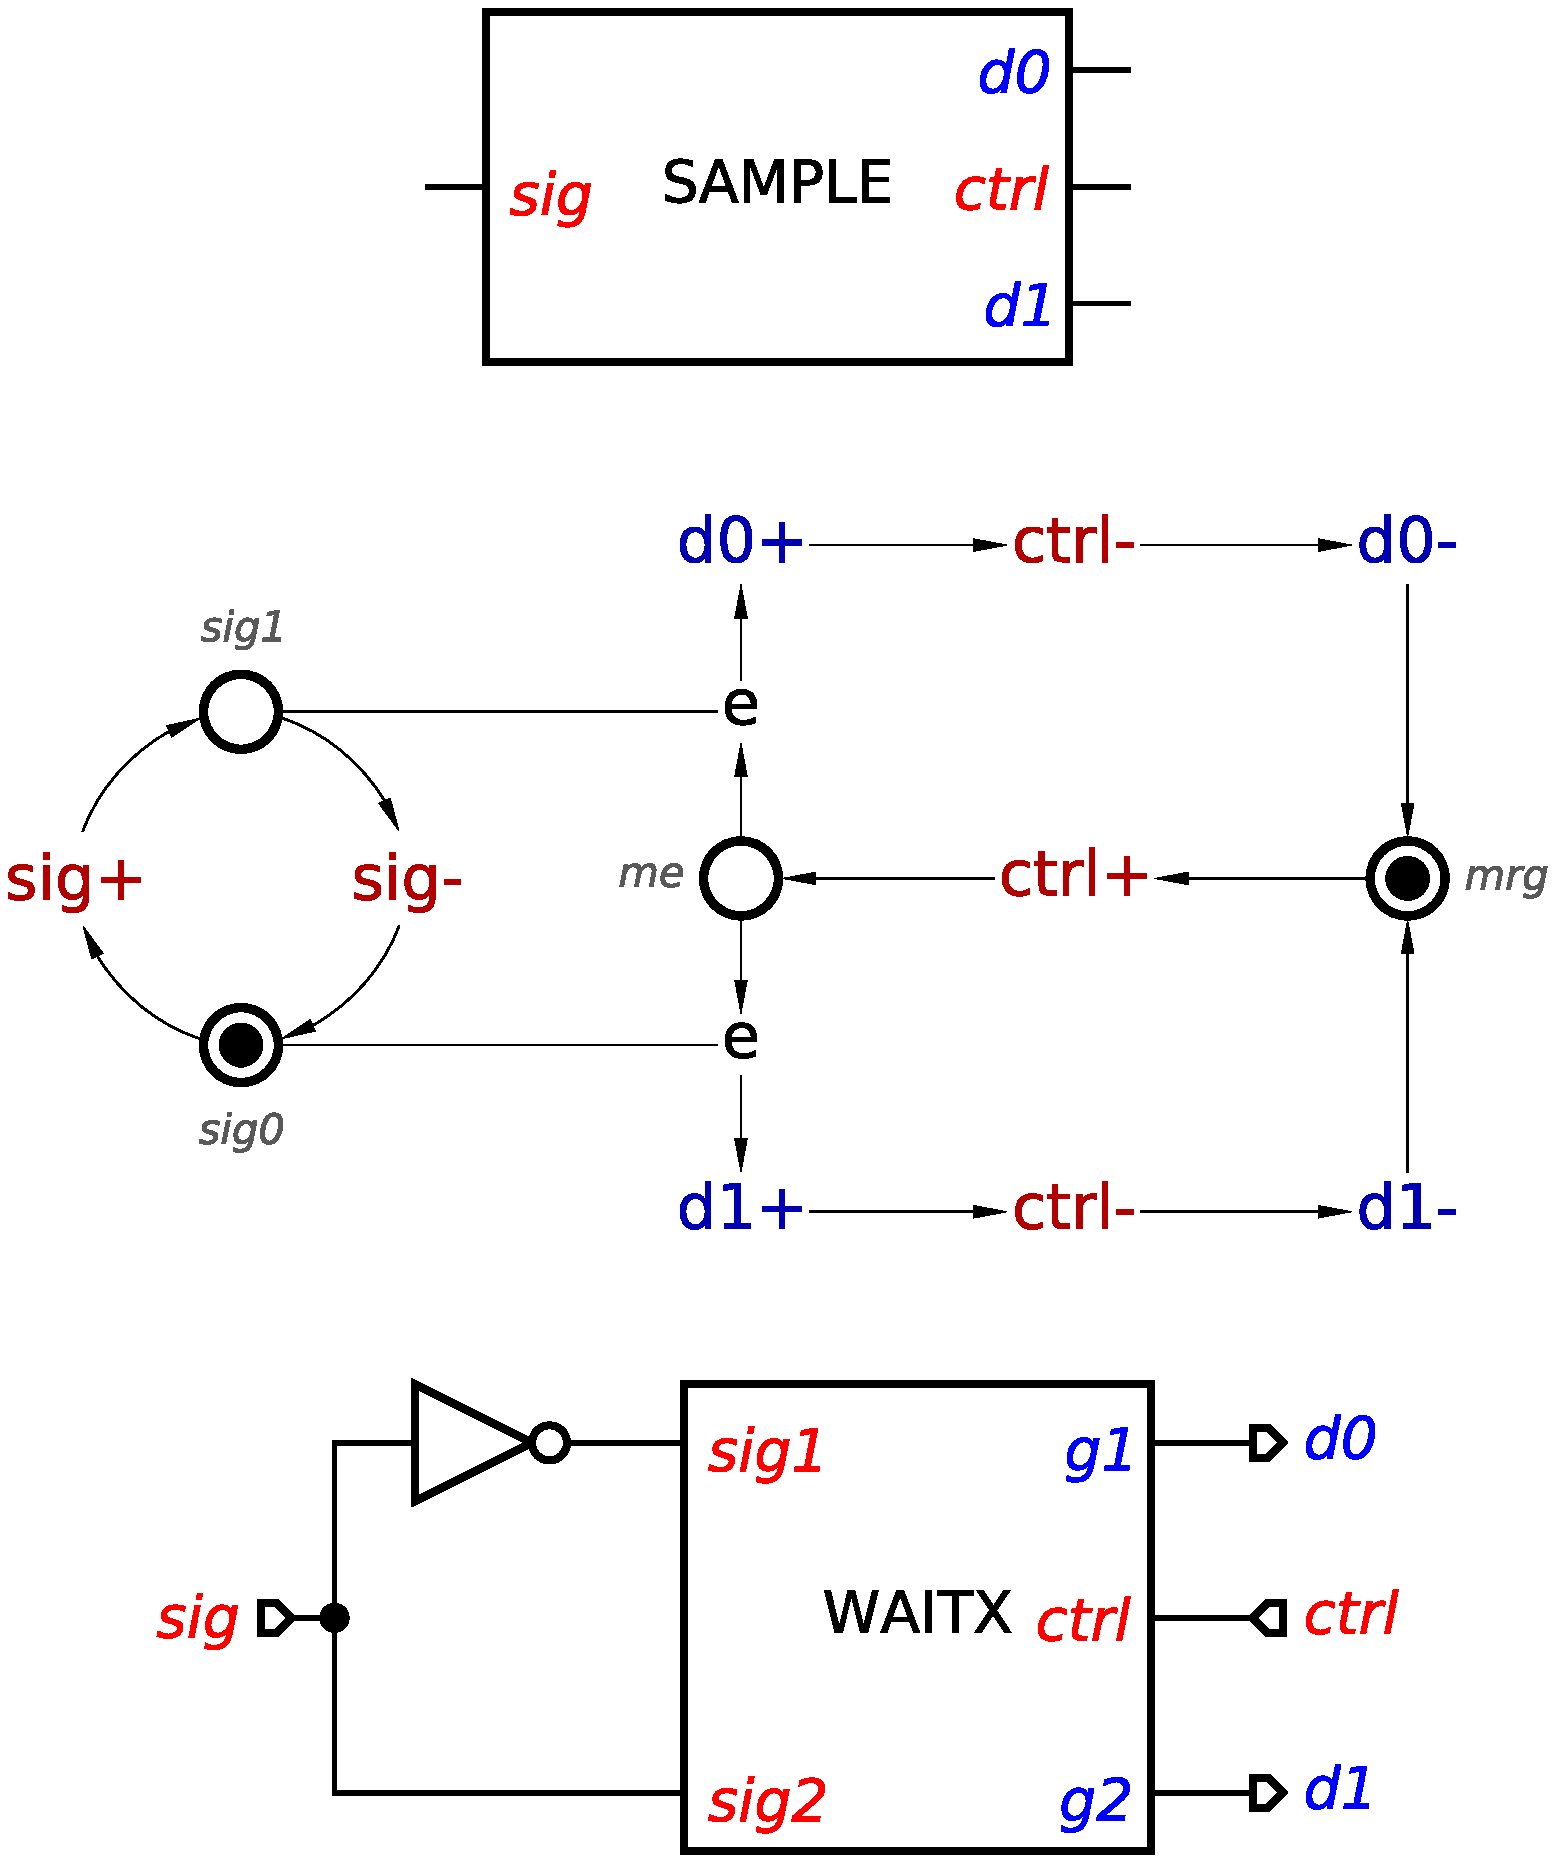
\includegraphics[scale=0.23]{fig/SAMPLE.pdf}
    \caption{\textsf{SAMPLE}: block diagram, specification and implementation.}
    \label{fig:sample}
    \vspace{-6mm}
\end{center}
\end{figure}

The purpose of the \textsf{SAMPLE} element is to check whether the voltage on the input
\textsf{sig} is above the threshold, see Fig.~\ref{fig:sample}. The specification is similar
to that of \textsf{WAITX} but the two dummy transitions are controlled by conditions
corresponding to the state of the same signal.

The implementation is based on \textsf{WAITX} that decides which of the two inputs,
\textsf{sig} or its inverted version, becomes high first. Note that both inputs may be
high at the same time, e.g. during a transition of \textsf{sig}, in which case
\textsf{SAMPLE} is allowed to make an arbitrary decision.

\subsection*{\textsf{OM}}

The \emph{opportunistic merge} \textsf{OM} element~\cite{2015_mokhov_om} merges two
request-acknowledgement channels $\{\textsf{r1}/\textsf{a1}, \textsf{r2}/\textsf{a2}\}$
into one $\textsf{r}/\textsf{a}$ and can opportunistically bundle requests from different
input channels if they arrive sufficiently close to each other.

Fig.~\ref{fig:om}(middle) clarifies the difference between the standard \emph{merge}
element~\cite{1999_greenstreet_merge} and \textsf{OM}. The conceptual state graph of
the merge element is shown on the left. Note that the bottom state of the graph is not
persistent: outputs \textsf{a1} and \textsf{a2} disable each other, hence this is a
decision-making element. The state graph for \textsf{OM}, shown on the right, has an additional
`opportunistic bundle' transition labelled by $\{\textsf{a1},\textsf{a2}\}$ that sends
acknowledgements to both input channels.

The intended application of \textsf{OM} is to handle concurrent (and potentially correlated) requests
from several clients to a kind of service that benefits all the clients simultaneously. Examples
include triggering an alarm by (any of) several sensors, re-charging of a shared DRAM, and
various kinds of power management~\cite{2017_sokolov_a4a}. The STG specification of
\textsf{OM}, as well as further implementation details can be found in~\cite{2015_mokhov_om}.

The input channels of \textsf{OM} are assumed to be hazard-free, but one can use one of the
synchronisation primitives presented in Section~\ref{sec-sync} to generate a clean hazard-free
handshake from a hazardous input signal, e.g. produced by an analog sensor.

\begin{figure}
\begin{center}
    \vspace{-1mm}
    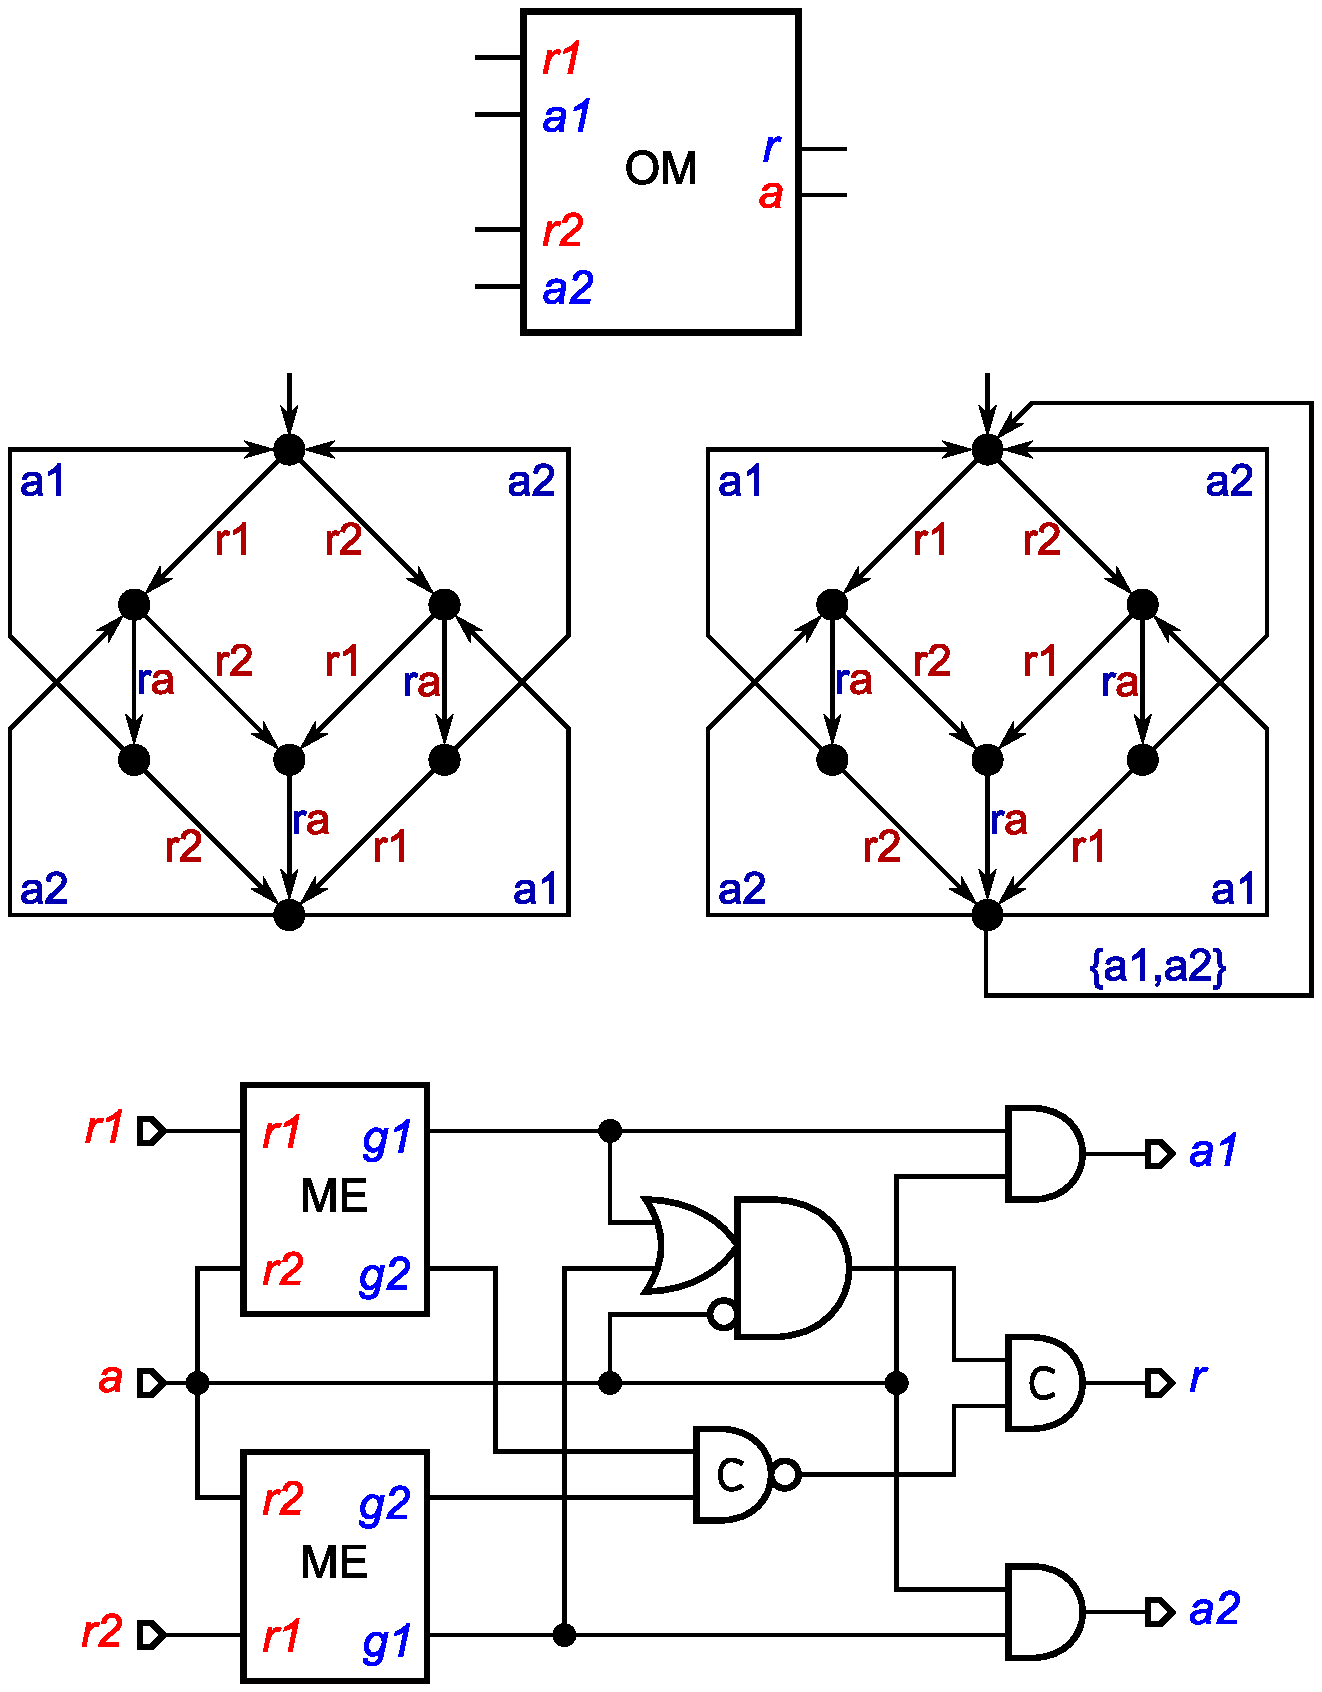
\includegraphics[scale=0.32]{fig/OM.pdf}
    \caption{\textsf{OM}: block diagram, conceptual state graphs,
    implementation.}
    \label{fig:om}
    \vspace{-6.5mm}
\end{center}
\end{figure}

\section{Conclusions}

The paper presented an overview of asynchronous arbitration primitives that can
be used as basic building blocks for the new generation of circuits and systems,
where resilient and efficient synchronisation between multiple clock and voltage
domains is an important challenge.
The primitives were developed using formal methods and are publicly
available~\cite{Arbitration_primitives_github}. Our current research is focused
on providing support for their automated insertion into asynchronous controllers
operating on the boundary with hazardous environment.

% them into the asynchronous design flow supported by \textsc{Workcraft}

\section*{Acknowledgements}
\vspace{-0.5mm}

This research was supported by EPSRC grant EP/L025507/1 ``A4A: Asynchronous design
for Analogue electronics''.

\bibliographystyle{unsrt}
\bibliography{publications}

\end{document}
